

% Colors
\definecolor{colorCellHighlight}{rgb}{0.85, 0.91, 0.97} % You can define Your own colors this way


% References
% Here You can choose the reference style

% ACM-style. Numeric references [1]. Alphabetical order.
% \usepackage[style=unitartucs/citations/numeric]{biblatex}

% IEEE-style. Numeric references [1]. Reference order.
\usepackage[style=unitartucs/citations/numeric,sorting=none]{biblatex}

% AMS-style. Trigraph references [ABC]. Alphabetical order.
% \usepackage[style=unitartucs/citations/alphabetic]{biblatex}

% APA-style. References with name and year (Koit 2010). Alphabetical order.
% \usepackage[style=unitartucs/citations/authoryear,uniquename=init]{biblatex}

\addbibresource{english/references.bib} % This file contains your bibliography entries


% Metadata
\title{Thesis Title}
\author{Author's Name}
\date{2024}
\supervisor{Supervisor's Name\degree{degree} \and Co-Supervisor's name\degree{degree}}
\curriculum{Computer Science Curriculum}
\thesis{Bachelor's Thesis (9 ECTS)}
\keywords{Layout, formatting, template}


% Here begins the document

\begin{document}

\maketitle

\linespread{1.45} \selectfont

\newpage
\pdfbookmark[1]{\infoname}{info} % Lisame infolehe PDF-faili järjehoidjatesse.

% Eesti keeles info.
\begin{infoEst}
\begin{abstract}
Siia kirjutage oma lõputöö lühikokkuvõte. See võib lühidalt teemasse sisse juhatada, kuid peaks enamikus katma ära Teie lõputöö sisu. Seda lugedes peaks olema üheselt selge, millest Teie lõputöös lugeda võib. Hea on näiteks kirjutada eesmärgi, meetodi, tulemuste ja järelduste kohta. Bakalaureusetöö korral võiksid nii eesti kui inglise keeles olevad lühikokkuvõtted mahtuda ühele leheküljele. Magistritöö või vajaduse korral võib eesti ja inglise keeles olevad osad kirjutada eraldi lehekülgedele. Mõelge oma tööd kirjeldavad võtmesõnad ning leidke CERCS kood(id).
\end{abstract}

\keywords{\@keywords}
\cercs{KOOD Koodi nimi}

% Koodid leiate: https://www.etis.ee/Portal/Classifiers/Index/26
% Nt: P170 Arvutiteadus, arvutusmeetodid, süsteemid, juhtimine (automaatjuhtimisteooria)
% Nt: P175 Informaatika, süsteemiteooria

\end{infoEst}


% Inglise keeles info.
\begin{infoEng}
\begin{abstract}
Write here the abstract of your work. The abstract could provide a brief introduction to the topic but should, in the majority, cover Your thesis work. When reading the abstract, it should become clear what can be read about in the rest of Your thesis. It is good to write about the purpose of the thesis, method(s), results, and findings of Your work. For a bachelor’s thesis, both the Estonian and English abstracts should fit into a single page. For a master’s thesis or when necessary, the Estonian and English sections of this page could be on separate pages. Come up with good keywords for Your work and find your CERCs code(s).
\end{abstract}

\keywords{Layout, formatting, template}
\cercs{CODE Code name in English}

\end{infoEng}

\newpage
\newpage
\pdfbookmark[1]{Visual Abstract}{visualsummary} % Adding the file to PDF bookmarks
\section*{Visual Abstract}

\begin{figure}[ht]
    \centering
    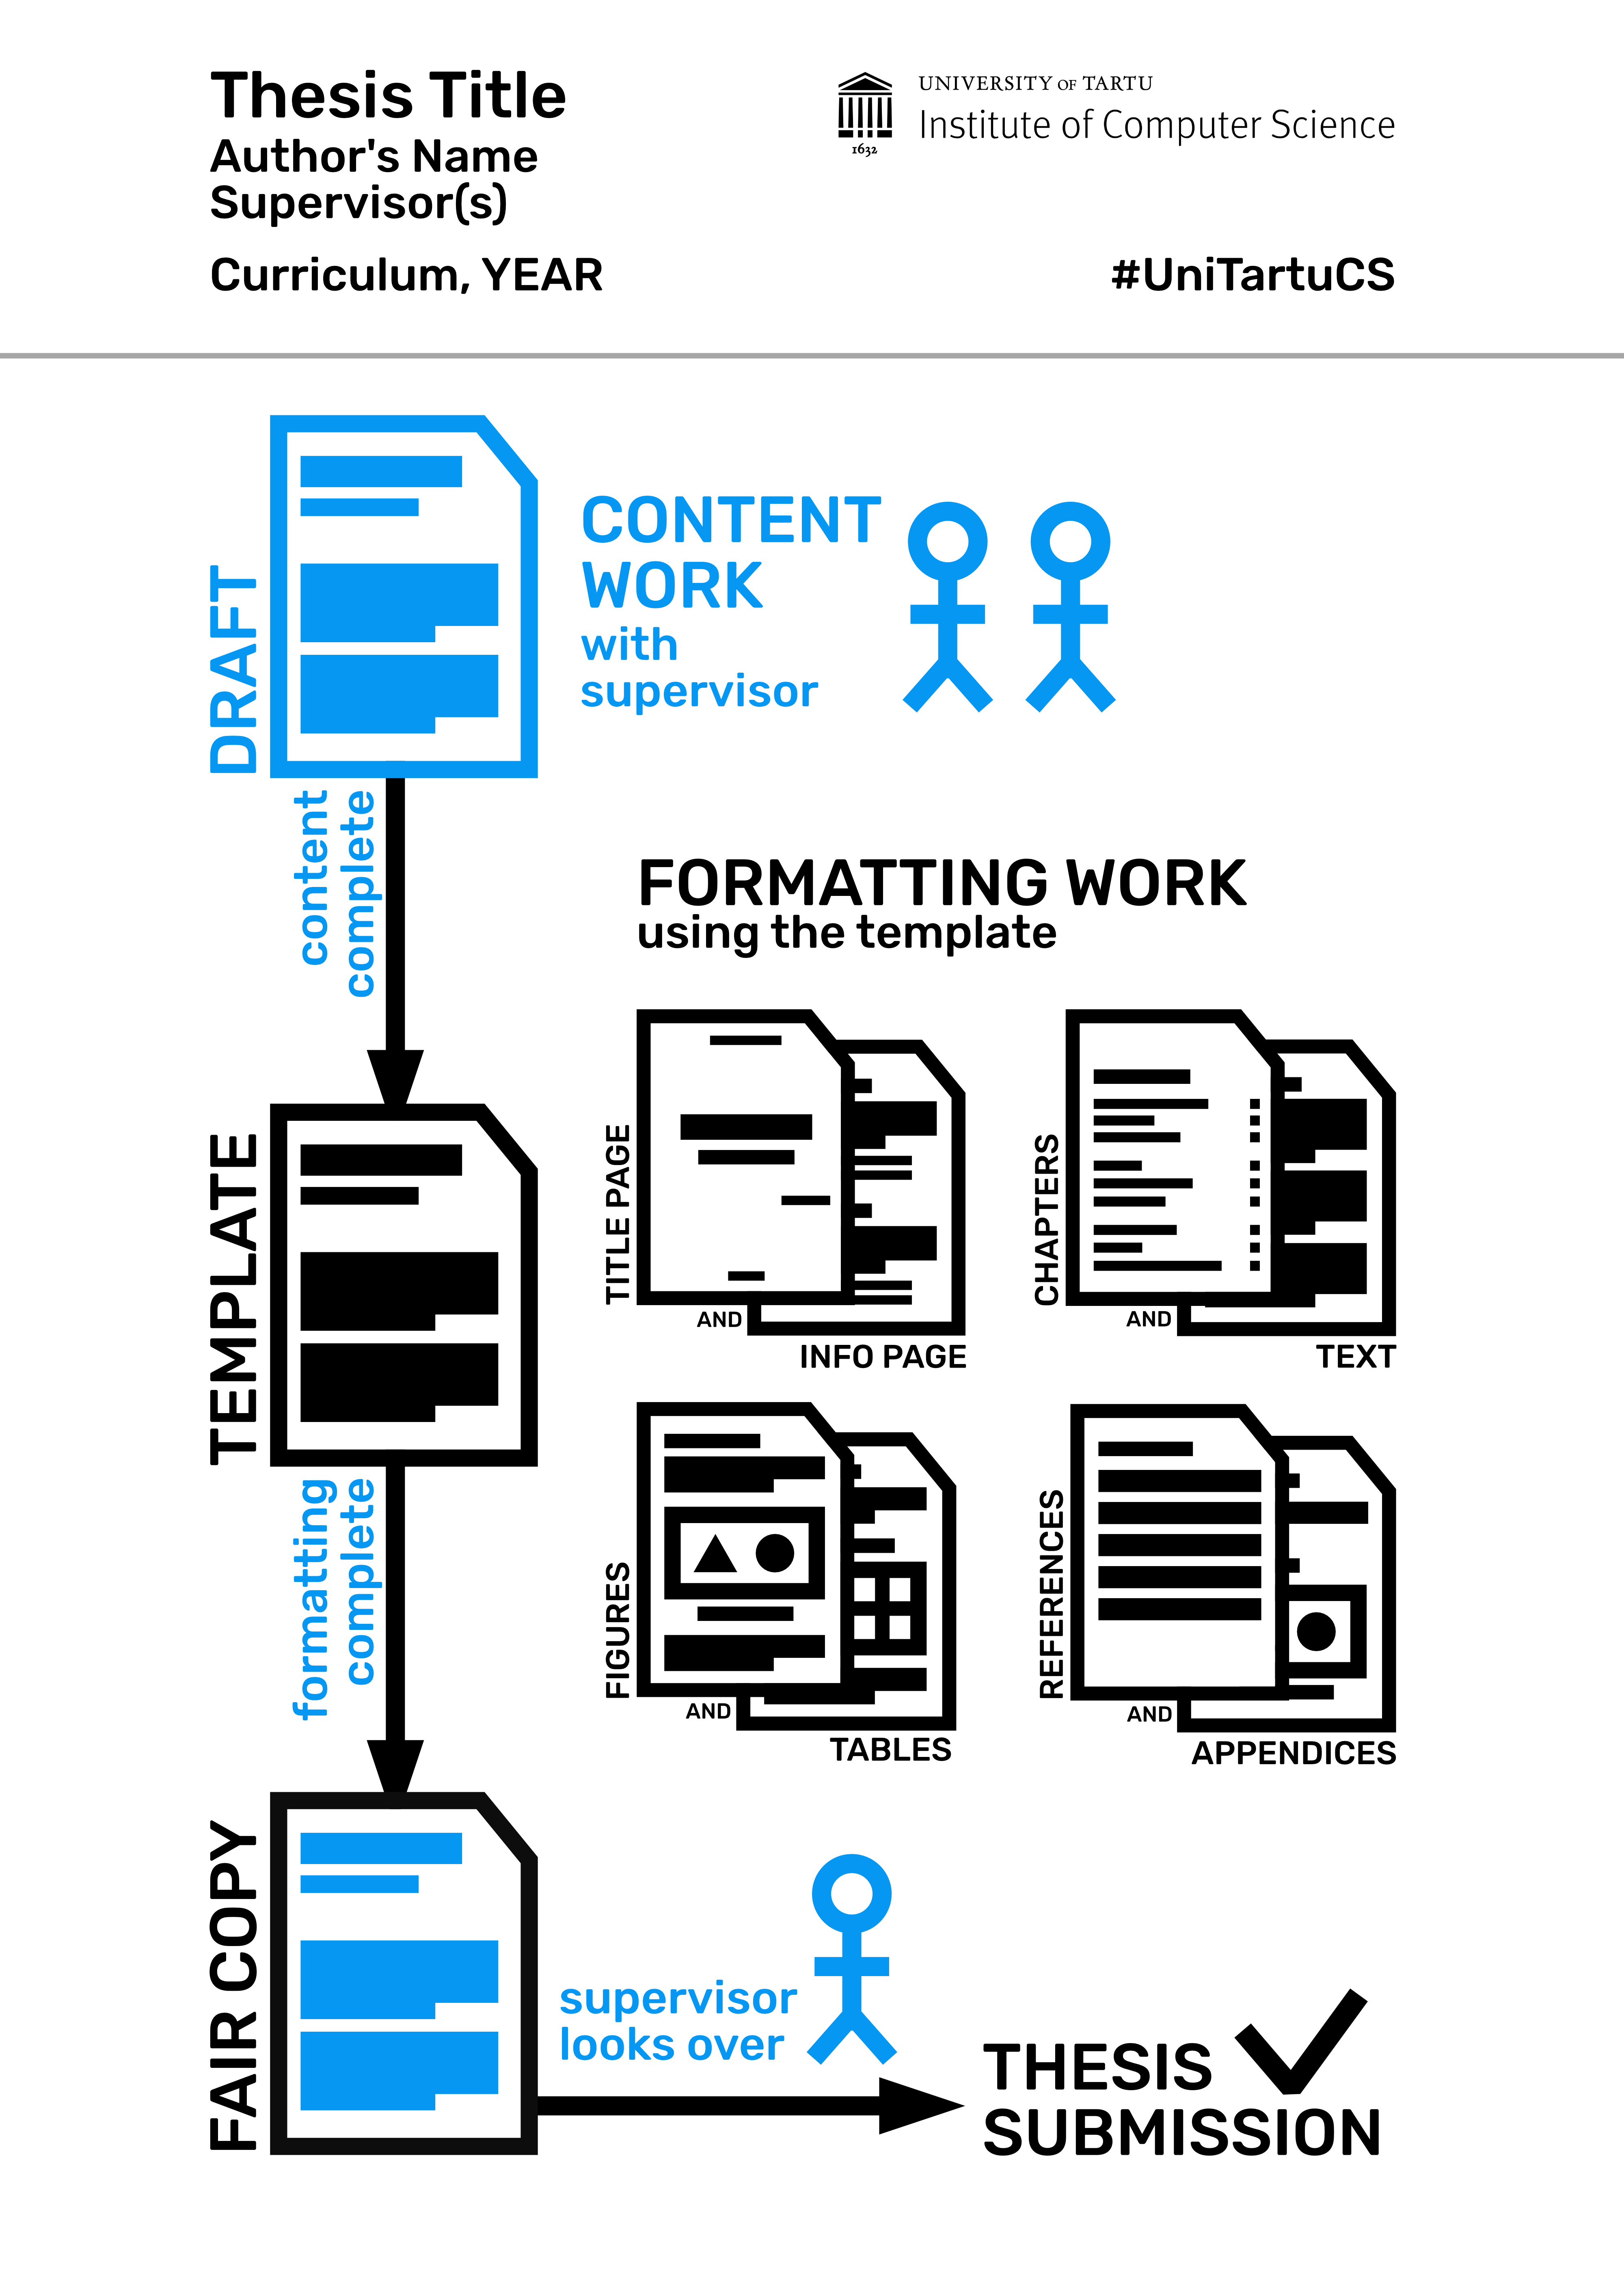
\includegraphics[width=0.85\textwidth]{figures/Figure0-VisualAbstract.png}
    \label{fig:visual-abstract}
\end{figure}

\newpage


\tableofcontents

\section{Introduction} \label{Introduction}

% Justification for the choice of topic
Autonomous driving systems promise to revolutionize transportation by increasing road safety, improving traffic efficiency, and reducing emissions \cite{litmanAutonomousVehicleImplementationb}.
% actuality
Autonomous driving systems are complex systems equipped with multi-sensor perception, integrating data from various sources. Autonomous driving systems should be capable of operating in various environments under diverse weather conditions. Autonomous vehicles are not yet ready, and mistakes or technical failures can cause accidents and undermine public trust.

% novelty
Autonomous driving systems heavily rely on deep learning for multiple perception tasks. Object detection is foundational among these tasks. In spite of the significant progress in this area, there is still a need for an effective and efficient general model architecture that is capable of understanding input from multiple sensors and is robust.

% Overview Theoretical Background -- background information to contextualize the problem
% review of state of the art solutions

Simple still-image detectors \cite{} cannot be applied to video data, because it contains challanges such as motion blur, occlusion etc.. Another approaches \cite{hanSeqNMSVideoObject2016, kangTCNNTubeletsConvolutional2018, kangObjectDetectionVideo2016} integrate a postprocessing after object detection improve results but those solutions are not end-to-end solutoins.

Another line of approaches \cite{Lu_2017_ICCV, xiaoVideoObjectDetection2018} leverages a second model to integrate motion and temporal information during training. 


% Problem statement -- if necessary, it should include the posed hypothesis/hypotheses, research questions, and subject of research

All of those detection pipelines for video object detection are over sophisticated, requiring many hand-crafted components, not capable of handling other modalities than images.

% Purpose of the Thesis -- overall aim and objective of the research, "why" of the research—why are you conducting this study?

In this thesis, our goal is to present a noval recurrent architecute we call Recurrent Perceiver inspired by Perceiver arhitecture. We present a training framework to asses robastness of the model.
Our main contributions are as follows:

\begin{itemize}
\item We propose a Recurrent Perceiver architecture. By unrolling it in time, the model can be interpreted as a recurrent neural network (RNN). Furthermore, the model supports multiple sensory inputs.
\item We propose a task to predict object center points and introduce custom-created benchmarks, which we call "detection-moving-mnist-easy," for evaluating this task.
\item We designed an experiment to simulate degraded input scenarios for single or multi-sensor (camera) setups. We evaluate the proposed Recurrent Perceiver, demonstrating that our training procedure with omitted input consistently achieves improved performance compared to training without dropout.
\end{itemize}

% [//]: # (The description of the structure of the thesis by chapter)

% A brief section giving background information may be necessary, especially if your work spans two or more traditional fields. That means that your readers may not have any experience with some of the material needed to follow your thesis, so you need to give it to them. A different title than that given above is usually better; e.g., "A Brief Review of Frammis Algebra.

Section~\ref{Background} gives background information about autonomous driving system architecture and overviews relevant video object detection approaches, and introduces original Perceiver model achitecture. Section~\ref{Methods} presents a noval Recurrent Perceiver architecture, presents benchmark used for training and testing, and explains training procedure. Section~\ref{Experiments} explains experiments and presents results.




% a short overview of appendices including the content of attached materials
% TODO

% TODO: Question where should i put it?
% This thesis was written using the Overleaf1 text editor. The text was checked with the
% Grammarly2 writing assistant to catch typos and other grammatical errors.
\section{Formatting}  \label{formatting}
Many different tools, some of which You might not even be aware of, will be used to format Your thesis. As good formatting makes up 25\% of Your thesis grade, it is important to take it seriously and allocate sufficient time. Especially if You have not previously formatted documents of that size that well or learned the use of corresponding tools. This chapter looks at the formatting principles for different parts of the thesis.

\subsection{The Title and Info Pages}
The very first page – the title page – is already formatted in this template. The title page must include the curriculum You plan to graduate from (including the educational institution and the institute), thesis title, kind and volume corresponding to the level of studies, Your name, the names (and, optionally, the academic degrees) of Your supervisors, publication location, and year. The information that goes to your title page must be entered into the specific fields in the file \path{thesis.tex}. Be sure to check the corresponding information. For example, if You decide to add the academic degrees of Your supervisors, check if an abbreviation is MSc (Master of Science) or MA (Master of Arts). The degrees differ depending on the curricula.

The info page (file \path{0-info.tex}), which follows Your title page, includes the abstract, keywords, and CERCS codes of Your work. The abstract should give an overview of everything done during Your work. For example, if three of Your content chapters thoroughly describe the different processes and results of Your work, then that should be readable from Your abstract. Concentrate on mentioning in the abstract what You did that can be read about in the thesis.

Keywords are the different terms and names that designate important aspects of Your work. To come up with keywords, You should think about Your work generally. What important terms come to Your mind if You think about Your work as a whole? For inspiration, it is good to check out the keywords of previous theses made on similar topics. Joonis~\ref{fig:keywords} shows the word cloud of keywords from the theses defended at the Institute of Computer Science in 2015–2020\footnote{\url{https://cglearn.eu/theses/top}}.

\begin{figure}[ht]
    \centering
    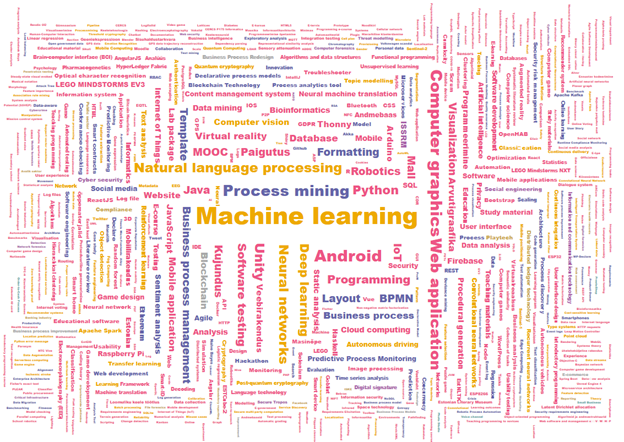
\includegraphics[width=\textwidth]{figures/Figure1-Keywords.png}
    \caption{The word cloud of keywords from theses defended at the Institute of Computer Science in 2015–2020.}
    \label{fig:keywords}
\end{figure}

Besides the keywords, You also need to assign a Common European Research Classification Scheme (CERCS) code to Your work. These codes classify research areas. Often, it can be hard to classify a thesis using a specific classifier. Still, You must find a classifier that Your work fits under the best. You can use several CERCS codes. The classifiers are on the Estonian Research Information System’s web page: \url{https://www.etis.ee/Portal/Classifiers/Index/26}.

After the info page, You can also add a visual abstract to Your work. That will be a single figure that efficiently describes the process and results of Your work. The figure has to include the information listed in the Guidelines for preparing and grading of graduation theses at the Institute of Computer Science of the University of Tartu document. When using the institute’s logo, respect its protected area – it must have the height of the house of free space around it. The visual abstract is helpful to add, as it quickly conveys the nature of Your work to the reader. You can reuse the graphics later on Your defense slides and when popularizing Your work.

\subsection{Structure}
It is essential for the reader of Your work that Your document is structured logically and clearly. Good titles and reasonable content sectioning to chapters and sub-chapters guide the reader through Your thesis.

\subsubsection{Titles}
Both the thesis title itself and the chapter titles should be concise and on-point. Long titles could carry too many ideas within themselves, and You can lose Your reader already at the title. The main title of the thesis should maximally fit on two lines.

In English, the words in titles start with capital letters. There are different styles, but generally, all the words besides pronouns should start with a capital letter. It is good to use the Capitalize My Title tool: \url{https://capitalizemytitle.com/}

In Estonian, however, only the very first letter of the title is capitalized, and the rest of the words are written just like regularly.

Punctuation should be avoided in titles. Depending on the nature of Your work, an em or en dash could be reasonable. For example, if You have created a software product, it is good to mention the product's name in the title, followed by a longer dash and a description of its unique value. On the other hand, a sentence with commas or question marks would not fit as a title.

These principles also apply to the titles of Your chapters, which are called headings. The content chapter headings start with numbers. It is up to You if You start the numbering from the Introduction chapter and end it with the Conclusion chapter or leave these two chapters unnumbered. In this template, the Introduction and Conclusion chapters are also numbered. The Conclusion chapter is followed by unnumbered sections called References and Appendices. For different appendices, it is reasonable to use some numbering again. To number the appendices, You can use Roman numerals (Appendix I, Appendix II) or capital letters (Appendix A, Appendix B).

The subchapter numbering includes the number from the parent chapter. For example, the subchapters of chapter 2 are numbered 2.1, 2.2, etc. The dot mark after the entire numbering is used only in the first-level headings. Starting from the third-level headings, the numbering can be omitted. In this template, the heading styles (\verb|\section{...}|, \verb|\subsection{...}|, etc) provide the correct numbering.

\subsubsection{Table of Contents}
At the beginning of Your work, after the info page and visual summary, but before the first chapter, there is the Table of Contents. Capable text editing software generates the Table of Contents automatically. In this template, the table of contents is created by the command \verb|\tableofcontents|. That command generates the table of contents automatically based on the sections/headings (\verb|\section{...}|, \verb|\subsection{...}| jne) of the document.

\subsection{Text}
The alignment of the thesis text must be justified (straight rug from both left and right). Justified alignment can create a situation when the spacing between words in one line is visually too much. In such cases, the line can be hyphenated to fix the visually bothersome spacing. Many text editors have automatic hyphenation capabilities, but these are prone to over-hyphenation. In this template, the automatic hyphenation is minimized and the package \verb|microtype| ensures that the spacing between the words would not get too large. Having hyphenated words hinders the readability of the text, so hyphenation should be used minimally. One should avoid situations when multiple subsequent rows are hyphenated.

The guidelines for preparing and grading of graduation theses at the Institute of Computer Science of the University of Tartu document presents many text formatting rules. For example, the line spacing of text should be in the range 1.0-1.5. This template uses 1.4 line spacing which visually corresponds to the 1.5 line spacing of Microsoft Word.

It is possible to use italics (\verb|\emph{...}|), bold (\verb|\textbf{...}|), or other text formatting tools to emphasize some terms or ideas in Your text. However, it is good to use these tools sparingly so as not to make Your work visually too hectic.

When writing paragraphs, You should observe that there would not be a single lone word at the last row of the paragraph. This is called an orphan word, and it is not visually very good. Checking for orphan words or lines (an orphaned line of text at the beginning of a page that is followed by a new chapter or empty page) is something one should do as one of the last things when formatting their fair copy.

\subsection{Elements}
Many different elements like figures, tables, and code examples improve the appearance and reader’s understanding of Your thesis.

\subsubsection{Figures}
All the different images, be they plots, photographs, or screenshots, are labeled as figures. When adding an image, it should be labeled as a figure, numbered, and captioned. In the LaTeX template here, this is done by first adding or uploading the image to the \verb|figures| folder. Afterward the image can be used via the following code:

\begin{minted}[escapeinside=||]{tex}
\begin{figure}
    \centering
    \includegraphics[width=\textwidth]{figures/|\textbf{Figure1-Name.png}|}
    \caption{|\textbf{Figure caption text.}|}
    \label{fig:|\textbf{figureLabel}|}
\end{figure}
\end{minted}

The code above must include the correct file name with the file extension inside the \verb|figures| folder, a short caption text, and a short \emph{label} for cross-referencing the figure.

It should be clear from the caption what is depicted in the image. The caption is shown under the figure together with the element's label \emph{Figure} and an automatic number.

\begin{wrapfigure}{r}{0.33\textwidth}
    \centering
    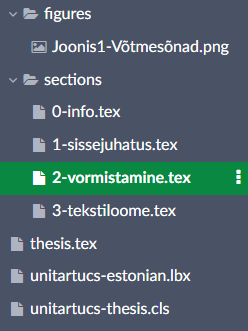
\includegraphics[width=0.33\textwidth]{figures/Figure2-figuresFolder.png}
    \caption{Template folders.}
    \label{fig:folders}
\end{wrapfigure}

You can add the images in the middle of the page or wrap text around them. To add a figure that is wrapped by text, write \verb|wrapfigure| instead of \verb|figure| in the example above. The figure's width could be, for example, \verb|width=0.33\textwidth|.

It is recommended to wrap the text around the image in situations where the image is about 1/3 of the width of the page. In other situations, it is likely better to have the image in the middle of the page without text wrapping.

When positioning the images, You have to be very careful not to scale the image unevenly. Both the vertical and horizontal scale of the image must change the same proportion. Typically this issue does not happen in LaTeX, but you should still consider it when working on the figures with other software.


We recommend creating a solid color palette when creating images. This means that You use the same colors (or course with the same semantics) for plots throughout Your thesis. A useful tool for creating a color palette is Coolors: \url{https://coolors.co/generate}. Depending on the situation, You need to consider that the chosen colors support the readability of Your plots. For example, You should not pick two very similar colors to represent different data points. Tamara Munzner has presented principles about data visualization in her talk Keynote on Visualization Principles~\cite{tamara_munzner_keynote_2012}. A good and cohesive color palette and style are crucial not only for plots but also for graphical elements added to screenshots or for figures in general.

\subsubsection{Tables}
A thesis can also include tables, in addition to figures. When adding tables, You should consider that reading very large tables is difficult and perhaps the data within them should rather be visualized on a plot. However, sometimes, it is important to represent the data as a table. Smaller tables can fit very nicely into the contents of a thesis. Larger tables can be added in the appendices (either in the Appendices section or as a file in the Accompanying Files archive).

The recommendations for figures are also the same for tables. The only difference is that the caption of a table goes above the table (the caption of a figure was below). For example, look at Table~\ref{tabel:elementDifferences}.

\begin{table}[htb!]
    \centering
    \caption{The differences between formatting figures and tables.}
    \label{tabel:elementDifferences}
    \begin{tblr}{width=1.0\textwidth, hlines, vlines,
                    colspec = { Q[r,font=\bfseries] Q[c] X[c] },
                    row{1} = {font=\bfseries},
                    cell{3}{2} = {bg = colorCellHighlight},
                }
                & Caption Placement     &   Content        \\
    Figure      & Below                 &   Images, graphs, photographs, screenshots     \\
    Table       & Above                 &    Data       \\
    Code Example& Below or absent       &    Program code, psudocode       \\
    \end{tblr}
\end{table}

The table \ref{tabel:elementDifferences} above is created with the following code:
\begin{minted}{tex}
\begin{table}[htb!]
    \centering
    \caption{The differences between formatting figures and tables.}
    \label{tabel:elementDifferences}
    \begin{tblr}{width=1.0\textwidth, hlines, vlines,
                    colspec = { Q[r,font=\bfseries] Q[c] X[c] },
                    row{1} = {font=\bfseries},
                    cell{3}{2} = {bg = colorCellHighlight},
                }
            & Caption Placement & Content                             \\
    Figure  & Below             & Images, graphs, photos, screenshots \\
    Table   & Above             & Data                                \\
    Code    & Below or absent   & Program code, psudocode             \\
    \end{tblr}
\end{table}
\end{minted}

That code is similar to the code for figures from before but has two environments. First, there is the \verb|table| environment which includes the caption preceeding the table. Then comes the \verb|tblr| environment that includes the table itself. In this case, the width of the table is the full width of the page \verb|1.0\textwidth| and the table has all the borders with \verb|hlines| and \verb|vlines|. The cells are created such that the first two are tight (\verb|Q|) and the last one has all the leftover space (\verb|X|). The cells are aligned such that the first one is right-aligned \verb|r| and the other ones center-aligned \verb|c|. The first column and row are written in bold and the cell with index (3,2) is colored light blue.

\subsubsection{Code}
When You bring examples of program code, You should use a monospace font. You should pick one and use it cohesively throughout Your thesis text. Examples of these are Consolas and \texttt{Courier New}. This template uses the \verb|fontspace| package that has the \texttt{Courier New} font\footnote{\url{https://www.overleaf.com/learn/latex/Questions/Which_OTF_or_TTF_fonts_are_supported_via_fontspec\%3F}}.

The formatting of code examples is not as regulated as figures and tables. Brief code examples can be written inside paragraphs. For example, one can write that declaring a variable and assigning a value can be done with code \verb|var a = 10;|. For longer code examples, You should create a separate block like this:

\begin{minted}{javascript}
function add(a, b) {
    return a + b;
}
\end{minted}

The example above uses the \verb|minted| environment from the \verb|minted| package. That environment is configured to add a border around the paragraph containing the code example and uses a monotype font. The \verb|minted| environment can also color the code of certain programming languages to make the code more readable\footnote{\url{https://www.overleaf.com/learn/latex/Code_Highlighting_with_minted\#Reference_guide}}. The text surrounding the code block must address the code example in a sufficiently clear and helpful manner.

\subsubsection{Mathematical Equations}
Formatting mathematical equations is relatively easy in LaTeX. To write a short equation inside regular text, the equation must be surrounded with \verb|$|-signs. For example, an equation descirbing addition is $a+b=c$. For a larger equation, the equation must be added inside the \verb|equation| environment.
\begin{equation}
    \frac{a + b}{c} = d
    \label{eq:abcd}
\end{equation}

The example above is created with the following code:
\begin{minted}{tex}
\begin{equation}
    \frac{a + b}{c} = d
    \label{eq:abcd}
\end{equation}
\end{minted}

As seen, an equation can also have a short label, it gets an automatic number and the label can be used to reference the equation from the text. For example, the example above in this template has a number ~\ref{eq:abcd}.

\subsection{References}
Correctly citing Your sources is very important in Your work. Failure to do so may result in academic fraud, which can cause Your thesis to get a negative review. This template explores three types of references. These are the cross‑references between the different elements of the thesis, the footnote references for the so‑called weak external references, and the main references, which are also called strong references.

\subsubsection{Ristviited}
All the figures, tables, and mathematical equations must be cross‑referenced from the text. The purpose of that rule is to ensure that the illustrative elements actually support Your content.  The added element must be connected with Your text and cross‑referenced in a suitable place. The element you cross-reference must have a label and to that label a cross-reference can be created with the command \verb|\ref{label}|. The reference will be a number that turns into a link inside the text (that remains when exporting a PDF). This means that the reader is taken to the referenced element when they click on the cross‑reference.

\subsubsection{Footnote References}
The external references can be called as weak and strong. This does not mean anything about their influence or usefulness to Your work. For some external sources, You must make a subjective decision if the reference will be rather the so-called weak or strong one. Weak references are, for example, references to Wikipedia pages, Stack Overflow posts, webpages of products, dictionaries, and private communication, where the referenced source is not a solid publication by a clear author. Generally speaking, all sorts of web references are usually weak references. However, a web reference to a blog post by a reputable author can be considered a strong reference.

The weak references should be formatted as footnote references. To do that, use the \verb|\footnote{...}| command and copy-paste the link into it. To make the link actually work, use the \verb|\url{...}| command around the link. For such references, it is not important to find the author (for example, with product websites, software documentation, or Wikipedia articles, it might not even be an easily deducible author). Typically, it is sufficient to add the link to the website where You got the cited information.

Such footnote references are very good, but in addition to those, Your work should be based on an adequate number of strong or main references.

\subsubsection{Main References}
In this template, the main references are such references that go to the References section at the end of Your thesis. That section is sometimes titled „Cited Literature“ or „Used Sources“. The strong references that go there are typically reputable publications by specific authors. For example, scientific papers, books, conference presentations, and theses, but these can also include blog posts or news articles. You should have a sufficient amount of strong references depending on the level of study that You are writing a thesis on. It is hard to say a specific number because it will depend on the nature of Your work, the quality of Your references, and how thoroughly You have used them. However, just two strong references would undoubtedly be too few for any level.

There are different reference styles commonly used in different fields. In Your thesis, You can pick a style that You prefer. In computer science, the ACM and IEEE numeric styles are common. In these styles, the source numbers are inside square brackets (for example, „[1]“, „[2]“, and so on), and these are used to reference a source in the text. In mathematics, the AMS trigraph style is popular. In that style, the square brackets contain the first letters or initials of the authors and part of the publication year (for example, „[Mun12]“). In social sciences, the popular style is APA, where the source is referenced by the author’s name and year in round brackets (for example, „(Munzner, 2012)“).

This template uses the \verb|biblatex| package for formatting the references. That package allows You to easily add your references, use them, and change the reference style. The file \verb|config.tex| is where You can choose which reference style you prefer in your thesis.

Besides referencing You also need to get the bibilographic entries of your references into LaTeX. It is recommended to use the Zotero\footnote{\url{https://www.zotero.org/}} citation source management tool. Zotero allows you to very easily collect sources and store data attributed to them (incl files and Your notes) into your personal database in the Zotero desktop application. Already when writing your draft in Google Docs, You can use Zotero to add references to correct places and format them.

When moving to LaTeX for formatting, you can export the necessary bibliographic entries from Zotero. For that, select the sources connected with your thesis and choose \emph{Export Items...} from the context menu (see Figure~{fig:zoteroContext}). From the popup window choose \verb|BibLaTeX| as the export format.

\begin{figure}[ht]
    \centering
    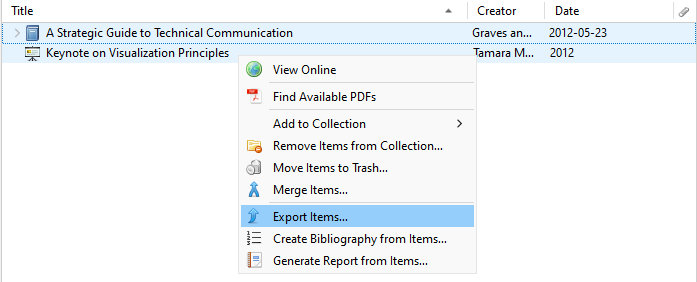
\includegraphics[width=\textwidth]{figures/Figure3-ZoteroBibliographyExport.png}
    \caption{The context menu of chosen sources in Zotero.}
    \label{fig:zoteroContext}
\end{figure}

After this, Zotero exports your chosen sources into a \verb|.bib|. The contents of that file you can copy into the \verb|references.bib| file in this environment. After that, referencing those sources in your text is already working. For each source, Zotero assigns a short label, which you can use to reference it. For example, the command \verb|\cite{tamara_munzner_keynote_2012}| has been used to create a reference to Tamara Munzner's lecture in this template.

The referenced scientific papers usually have Document Object Identifier (DOI) numbers. Specific DOI links\footnote{\url{https://dx.doi.org/}} (in the form doi.org/[number]) are generated from these. When referencing scientific papers, it is recommended to add the DOI links to the reference without the access date. When adding source links, ensure the links are correct and working. When You use the university proxy to access the papers, Your links directly on the browser’s address bar could be proxy links. Do not copy these into Your thesis. Ensure that Your reference links are clean and working, and, when possible, prefer the DOI links.

\subsection{Appendices}
The Appendices section in Your thesis follows the References section. In that part You can present larger tables or screenshots that do not fit in the main contents. Often, it is reasonable to present Your Glossary to define the jargon terms used in Your thesis. If You have created software during Your work, the Appendices section can also include the installation instructions and user manual. The section can be subsectioned and numbered in Your preferred way. For example, Appendix I: Glossary or Appendix B – User Manual, etc. There are many guides to creating a good user manual, but one example of writing technical texts is the textbook „A Strategic Guide to Technical Communication“ by Graves and Graves~\cite{graves_strategic_2012}.

One very important appendix is the description of the accompanying files. Together with the thesis document, You can also add an archived file. That archive file usually includes longer texts (for example, if Your user manual is very long, You need to include longer license texts for the user assets, the questionnaire used in Your study, etc.), larger files (for example, the measured raw data, their analysis files, audio and video recordings of the software or its testing, etc.), the created software, its source code, design concepts and other files created during Your work. Use one of the appendices to describe the contents of the accompanying files.

\subsection{License} \label{subchapter:license}
After the Appendix section, at the end of Your document, You must add a license to allow the  University of Tartu to store and distribute Your thesis. The text of that license is updated often and depends on whether Your work is classified or not. The newest texts are at the URL:  \url{https://adr.ut.ee/?page=pub_list_dynobj&desktop=57835&tid=70993&data_only=true&search=Otsi&field_100193_search_type=ANY&field_100193_text_search_value=ppimine}

The link above has the non-exclusive license as document number 30. In most cases, that license should apply to You. When Your work includes information that must not be published during some timeframe or even indefinitely, You need to write a corresponding application to the vice dean for academic affairs to use a limiting license. The application is in document number 32, and when the vice dean of academic affairs has approved Your application, You can use the corresponding limiting license from document number 31.

\subsection{Metadata}
Your thesis file includes metadata – data about the file itself. This template adds them automatically based on the fields you have written in the \verb|thesis.tex| file. You can see the metadata of a PDF file with the Acrobad Reader software, when you choose \emph{Document Properties} from the context menu of the opened document (see Figure~\ref{fig:metadata}). It is important that the metadata of your work correspond to reality.

\begin{figure}[ht]
    \centering
    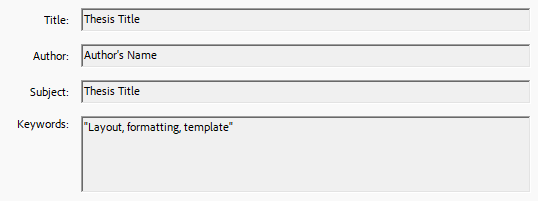
\includegraphics[width=0.8\textwidth]{figures/Figure4-Metadata.png}
    \caption{The metadata of the tempalte in Acrobat Reader.}
    \label{fig:metadata}
\end{figure}

It is recommended that You check through the rest of the metadata to ensure it is all good. For example, it has happened that the author of the file has not been the author of the thesis. This kind of contradiction creates suspicion about who has really authored the thesis document.

\section{Text Creation} \label{textCreation}
By the time You start using this template, You have likely completed its contents using a more comfortable and collaborative software like Google Docs. Starting formatting makes sense only when the contents of Your work no longer change much. Otherwise, the changes in the content may require doing the formatting part again. Still, some formatting-related recommendations are relevant a lot earlier than when formatting the draft to a fair copy.

\subsection{Chapters}
Your thesis chapters should be evenly balanced with each other. Because this template focuses on formatting, then that guideline is broken here (the previous chapter~\ref{formatting} is noticeably lengthier than this chapter~\ref{textCreation}). In Your work, all the chapters besides the Introduction and Conclusion should have a relatively even length. This principle also helps You not overdo a single part of Your work but spread Your attention to all the essential parts. What precisely these parts are depends on Your thesis type. The University of Tartu’s Institute of Computer Science’s thesis preparation and grading guidelines document defines a certain number of these types. The study or research group where You are doing Your thesis might define continuations of those types. Ensure that Your thesis document provides a balanced coverage of all Your chosen thesis type requires.

\begin{wrapfigure}{r}{0.33\textwidth}
    \centering
    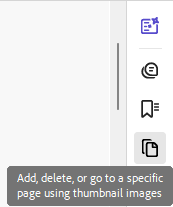
\includegraphics[width=0.33\textwidth]{figures/Figure5-AcrobatReaderMenu.png}
    \caption{The right-hand menu of Acrobat Reader.}
    \label{fig:acrobatReaderMenu}
\end{wrapfigure}
By the time Your thesis starts to take shape, it is useful to look at Your document as a whole. This can be done, for example, with the page order changing tool (\emph{Add, delete, or go to specific page using thumbnail images}) in the Acrobat Reader PDF viewer. The view from that tool shows You Your thesis as a whole. Just like if You would have printed out all of the pages and spread them across a desk. From that view, You see if all the different parts of the document are balanced and in visual equilibrium (see Figure~\ref{fig:acrobatReaderOverview}).

Seda saab teha näiteks Acrobat Reader PDF vaaturis lehekülgede järjekorra muutmise (\emph{Add, delete, or go to specific page using thumbnail images}) tööriistaga (vt joonis~\ref{fig:acrobatReaderMenu}). Tolle tööriista kuva näitab Teile tervet Teie tööd ülevaatlikult. Justkui oleksite oma töö välja printinud ja kõik lehed eraldi suure laua peale laotanud. Sellest ülevaatest Te näete, kas Teie erinevad töö osad on omavahel tasakaalus ja visuaalselt kooskõlas (vt joonis~\ref{fig:acrobatReaderOverview}).

\begin{figure}[t]
    \centering
    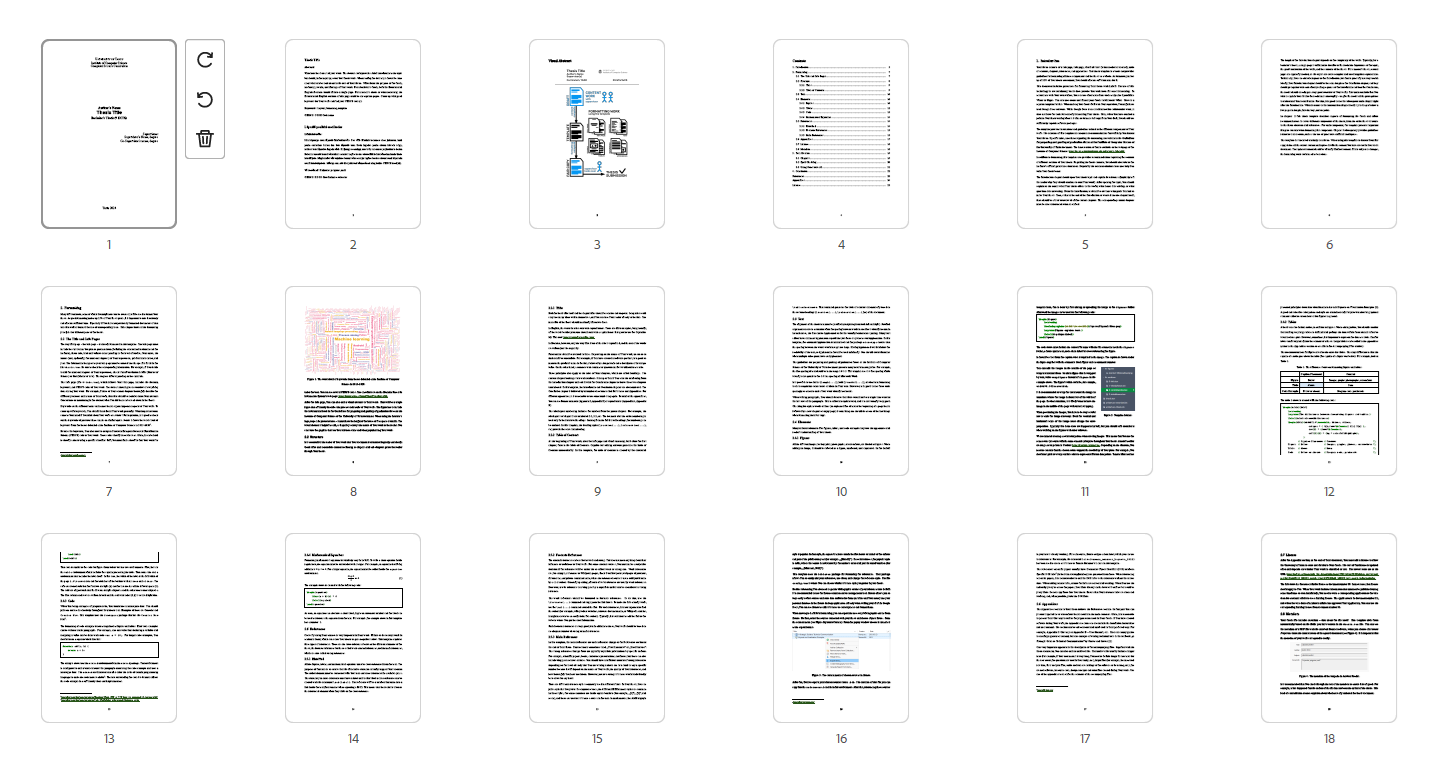
\includegraphics[width=\textwidth]{figures/Figure6-AcrobatReaderOverview.png}
    \caption{The overview of the thesis template in Acrobat Reader.}
    \label{fig:acrobatReaderOverview}
\end{figure}
he birds-eye view of the thesis also shows You if all the necessary places have text. For example, every chapter should start with a brief introductory text. This text must be after the   heading and before any subheadings. That introductory text usually explains why the corresponding chapter is necessary for Your work and what the reader can expect from the subchapters. In addition to that, the (sub)chapters could be woven together with connective sentences, and every bigger chapter could end with a conclusive paragraph. No chapter should start or end with any elements (figures, tables, code examples, equations) or a list. Your thesis text must be smooth to read.

\subsection{Spell Checking}
Microsoft Word’s speller, which You should turn on, comes in really handy when formatting Your fair copy. Having worked on Your draft a lot, You might have gotten used to looking at the same text over and over again; thus, noticing spelling mistakes Yourself might be quite difficult. There are spelling and proofing tools in Word for both the Estonian and English languages. Presenting a thesis that has grammatical errors can result in a lower grade.

Of course, You are also free to use tools that provide grammatical assistance, such as Grammarly, if You have access to such tools, and they make Your work more effective.

\subsection{Using Generative AI}
Using generative AI tools can also make Your work more effective. Here, their use for purely text editing purposes is focused on. When You have also used generative AI for content-related purposes (for example, to create Your questionnaire questions), You should definitely detail Your generative AI usage within the contents of Your thesis text. However, using it for editing Your thesis text is not content-related, so it will suffice to mention its use at the end of the Introduction chapter.

One good way to use a generative AI chatbot is to give it a paragraph of Your text and a prompt to make the specified academic text more readable. When doing that, You should read the result and correct it as needed. The AI chatbot might have mutated Your thoughts in the text, and You must restore them. Also, You might not personally agree with the specific style that AI has provided You and may want to keep tweaking it. The generative AI tools can very effectively help improve Your text flow, but You have to be very keen to ensure that the modified text still conveys Your thoughts and that You agree with the proposed writing style.

It is certainly not effective to use paragraphs that are solely generated by AI in Your thesis text. The author of the thesis is still You. This means that You are responsible for what is written in Your document. Typically, the text written by AI tends to be too general, overly illustrative and includes factual errors that a knowledgeable human author would not make. You do not want to put Yourself into a situation where You have to direct blame towards an AI chatbot due to issues in Your thesis text.

\section{Conclusion} \label{Conclusion}
This thesis template has given an overview and recommendations on various formatting and text creation techniques. For specific rules, it is useful to see the Guidelines for preparing and grading of graduation theses at the Institute of Computer Science of the University of Tartu document. Although this template focused on the LaTeX technology, the formatting rules and recommendations also apply to other capable text editors (for example, Microsoft Word, OpenOffice Writer, Pages, etc.). When creating a fair copy from Your draft, ensure that Your chosen text editor includes all the necessary tools. For example, Google Docs is not suitable for that work as it is missing several required tools presented in this template.

When formatting Your thesis, look at Your thesis document both as a whole (structure, balance, visual style) as well as individual components separately (info page, content elements, references, metadata). The different parts of Your work need different approaches. For example, to format the main references effectively, an external tool like Zotero might be useful. Formatting means not only positioning and cross-referencing an element but also the formatting of the element itself. For example, the plots in Your thesis must be well-designed and neatly formatted, just like the thesis itself. It is crucial to allocate enough time to study the tools and techniques to format Your thesis thoroughly.

Hopefully, this template helps You. To use this template, make a copy of it and delete or substitute all the content text. The pre-configured text styles should help You format Your draft to a fair copy. Certainly, look over Your document’s metadata and ensure they correspond to Your real thesis contents. Your supervisor can also be very helpful when it comes to thesis formatting. So, be active in asking them for help. Good luck with this last graded 25\% You do before submitting Your Thesis!

\clearpage
\printbibliography[heading=bibintoc]

\section*{Appendices} \label{appendices} \addcontentsline{toc}{section}{Appendices}

\subsection*{A. Training Hyperparameters} \label{Appendix:TrainingHyperparameters}

\begin{table}[htb!]
    \centering
    \caption{Hyperparameters used for training the RPerceiver model for bounding box prediction task.}
    \label{tab:training_params_bbox_20250505}
    \begin{tblr}{width=1\textwidth, hlines, vlines,
                   colspec = { l l X },
                   row{1} = {font=\bfseries},
                   colsep=3pt,
                  }
        Hyperparameter & Value & Description \\
        backbone & cnn & Backbone type \\
        batch\_size & 1 & Batch size for training \\
        bbox\_loss\_coef & 5 & L1 box coefficient \\
        eos\_coef & 0.1 & Relative classification weight of the no-object class \\
        epochs & 32 & Number of training epochs \\
        giou\_loss\_coef & 2 & GIoU box coefficient \\
        learning\_rate & 0.0001 & Learning rate \\
        learning\_rate\_backbone & 0.0001 & Learning rate \\
        num\_frames & 20 & Number of frames. \\
        object\_detection & True & Use object detection prediction head \\
        resize\_frame & 320 & Resize frame to this size \\
        scheduler\_step\_size & 18,28 & Scheduler step size \\
        set\_cost\_bbox & 5 & L1 box coefficient in the matching cost \\
        set\_cost\_class & 1 & Class coefficient in the matching cost \\
        set\_cost\_giou & 2 & giou box coefficient in the matching cost \\
        weight\_decay & 0.01 & Weight decay for optimizer \\
        weight\_loss\_bce & 1 & Weight loss binary cross entropy \\
        weight\_loss\_center\_point & 5 & Weight loss center point \\
    \end{tblr}
\end{table}

\begin{table}[htb!]
    \centering
    \caption{Hyperparameters used for training the RPerceiverMM model for center point task.}
    \label{tab:training_params_cp_20250505}
    \begin{tblr}{width=1\textwidth, hlines, vlines,
                   colspec = { l l X },
                   row{1} = {font=\bfseries},
                   colsep=3pt,
                  }
        Hyperparameter & Value & Description \\
        backbone & cnn & Backbone type \\
        batch\_size & 1 & Batch size for training \\
        bbox\_loss\_coef & None & L1 box coefficient \\
        eos\_coef & None & Relative classification weight of the no-object class \\
        epochs & 21 & Number of training epochs \\
        giou\_loss\_coef & None & GIoU box coefficient \\
        learning\_rate & 0.0001 & Learning rate \\
        learning\_rate\_backbone & 0.0001 & Learning rate \\
        num\_frames & 12 & Number of frames. \\
        object\_detection & None & Use object detection prediction head \\
        resize\_frame & None & Resize frame to this size \\
        scheduler\_step\_size & 18 & Scheduler step size \\
        set\_cost\_bbox & None & L1 box coefficient in the matching cost \\
        set\_cost\_class & None & Class coefficient in the matching cost \\
        set\_cost\_giou & None & giou box coefficient in the matching cost \\
        weight\_decay & 0.01 & Weight decay for optimizer \\
        weight\_loss\_bce & 1 & Weight loss binary cross entropy \\
        weight\_loss\_center\_point & 5 & Weight loss center point \\
    \end{tblr}
\end{table}

\clearpage
\subsection*{B. Model Hyperparameters} \label{Appendix:ModelHyperparameters}

\begin{table}[htb!]
    \centering
    \caption{Hyperparameters used for configuring RPerceiver model.}
    \label{tab:model_params_RPerceiver_20250505}
    \begin{tblr}{width=1\textwidth, hlines, vlines,
                   colspec = { l l X },
                   row{1} = {font=\bfseries},
                   colsep=3pt,
                  }
        Hyperparameter & Value & Description \\
        enc\_layers & 1 & Number of layers in Perceiver encoder \\
        enc\_nheads\_cross & 1 & Number of cross-attention heads \\
        hidden\_dim & 128 & Latent dimension size \\
        max\_freq & 10 & Maximum frequency for Fourier encoding \\
        nheads & 1 & Number of latent self-attention heads \\
        num\_freq\_bands & 6 & Number of frequency bands for Fourier encoding \\
        num\_queries & 16 & Number of latents, or induced set points, or centroids \\
        self\_per\_cross\_attn & 1 & Number of self-attention blocks per cross-attention block \\
    \end{tblr}
\end{table}

\begin{table}[htb!]
    \centering
    \caption{Hyperparameters used for configuring RPerceiverMM model.}
    \label{tab:model_params_RPerceiverMM_20250505}
    \begin{tblr}{width=1\textwidth, hlines, vlines,
                   colspec = { l l X },
                   row{1} = {font=\bfseries},
                   colsep=3pt,
                  }
        Hyperparameter & Value & Description \\
        enc\_layers & 1 & Number of layers in Perceiver encoder \\
        enc\_nheads\_cross & 1 & Number of cross-attention heads \\
        hidden\_dim & 128 & Latent dimension size \\
        max\_freq & 10 & Maximum frequency for Fourier encoding \\
        nheads & 1 & Number of latent self-attention heads \\
        num\_freq\_bands & 6 & Number of frequency bands for Fourier encoding \\
        num\_queries & 16 & Number of latents, or induced set points, or centroids \\
        self\_per\_cross\_attn & 1 & Number of self-attention blocks per cross-attention block \\
    \end{tblr}
\end{table}

\section*{License} \label{license} \addcontentsline{toc}{section}{License}
To here You must add a license that allows the University of Tartu to store and publish Your thesis. The newest license texts can be found at the following address:

\url{https://adr.ut.ee/?page=pub_list_dynobj&desktop=57835&tid=70993&data_only=true&search=Otsi&field_100193_search_type=ANY&field_100193_text_search_value=ppimine}

Please read chapter~\ref{subchapter:license} in this template to know what license You have to use on this page.


\end{document}



